\chapter{Аналитическая часть}

\section{Волновой процесс}

При каком-либо внешнем воздействии на поверхность воды (ветер, движение корабля, падение камня) частицы жидкости опускаются вниз, и водная поверхность становится вогнутой. Сила тяжести или сила поверхностного натяжения стремятся вернуть частицы в состояние равновесия. При этом частицы воды переходят это положение, и поверхность воды становится выпуклой. Движение передается от одних частиц к другим. Так на водной поверхности появляются волны. Волновой процесс показан на рисунке 1.1.

\begin{figure}[H]
	\begin{center}
		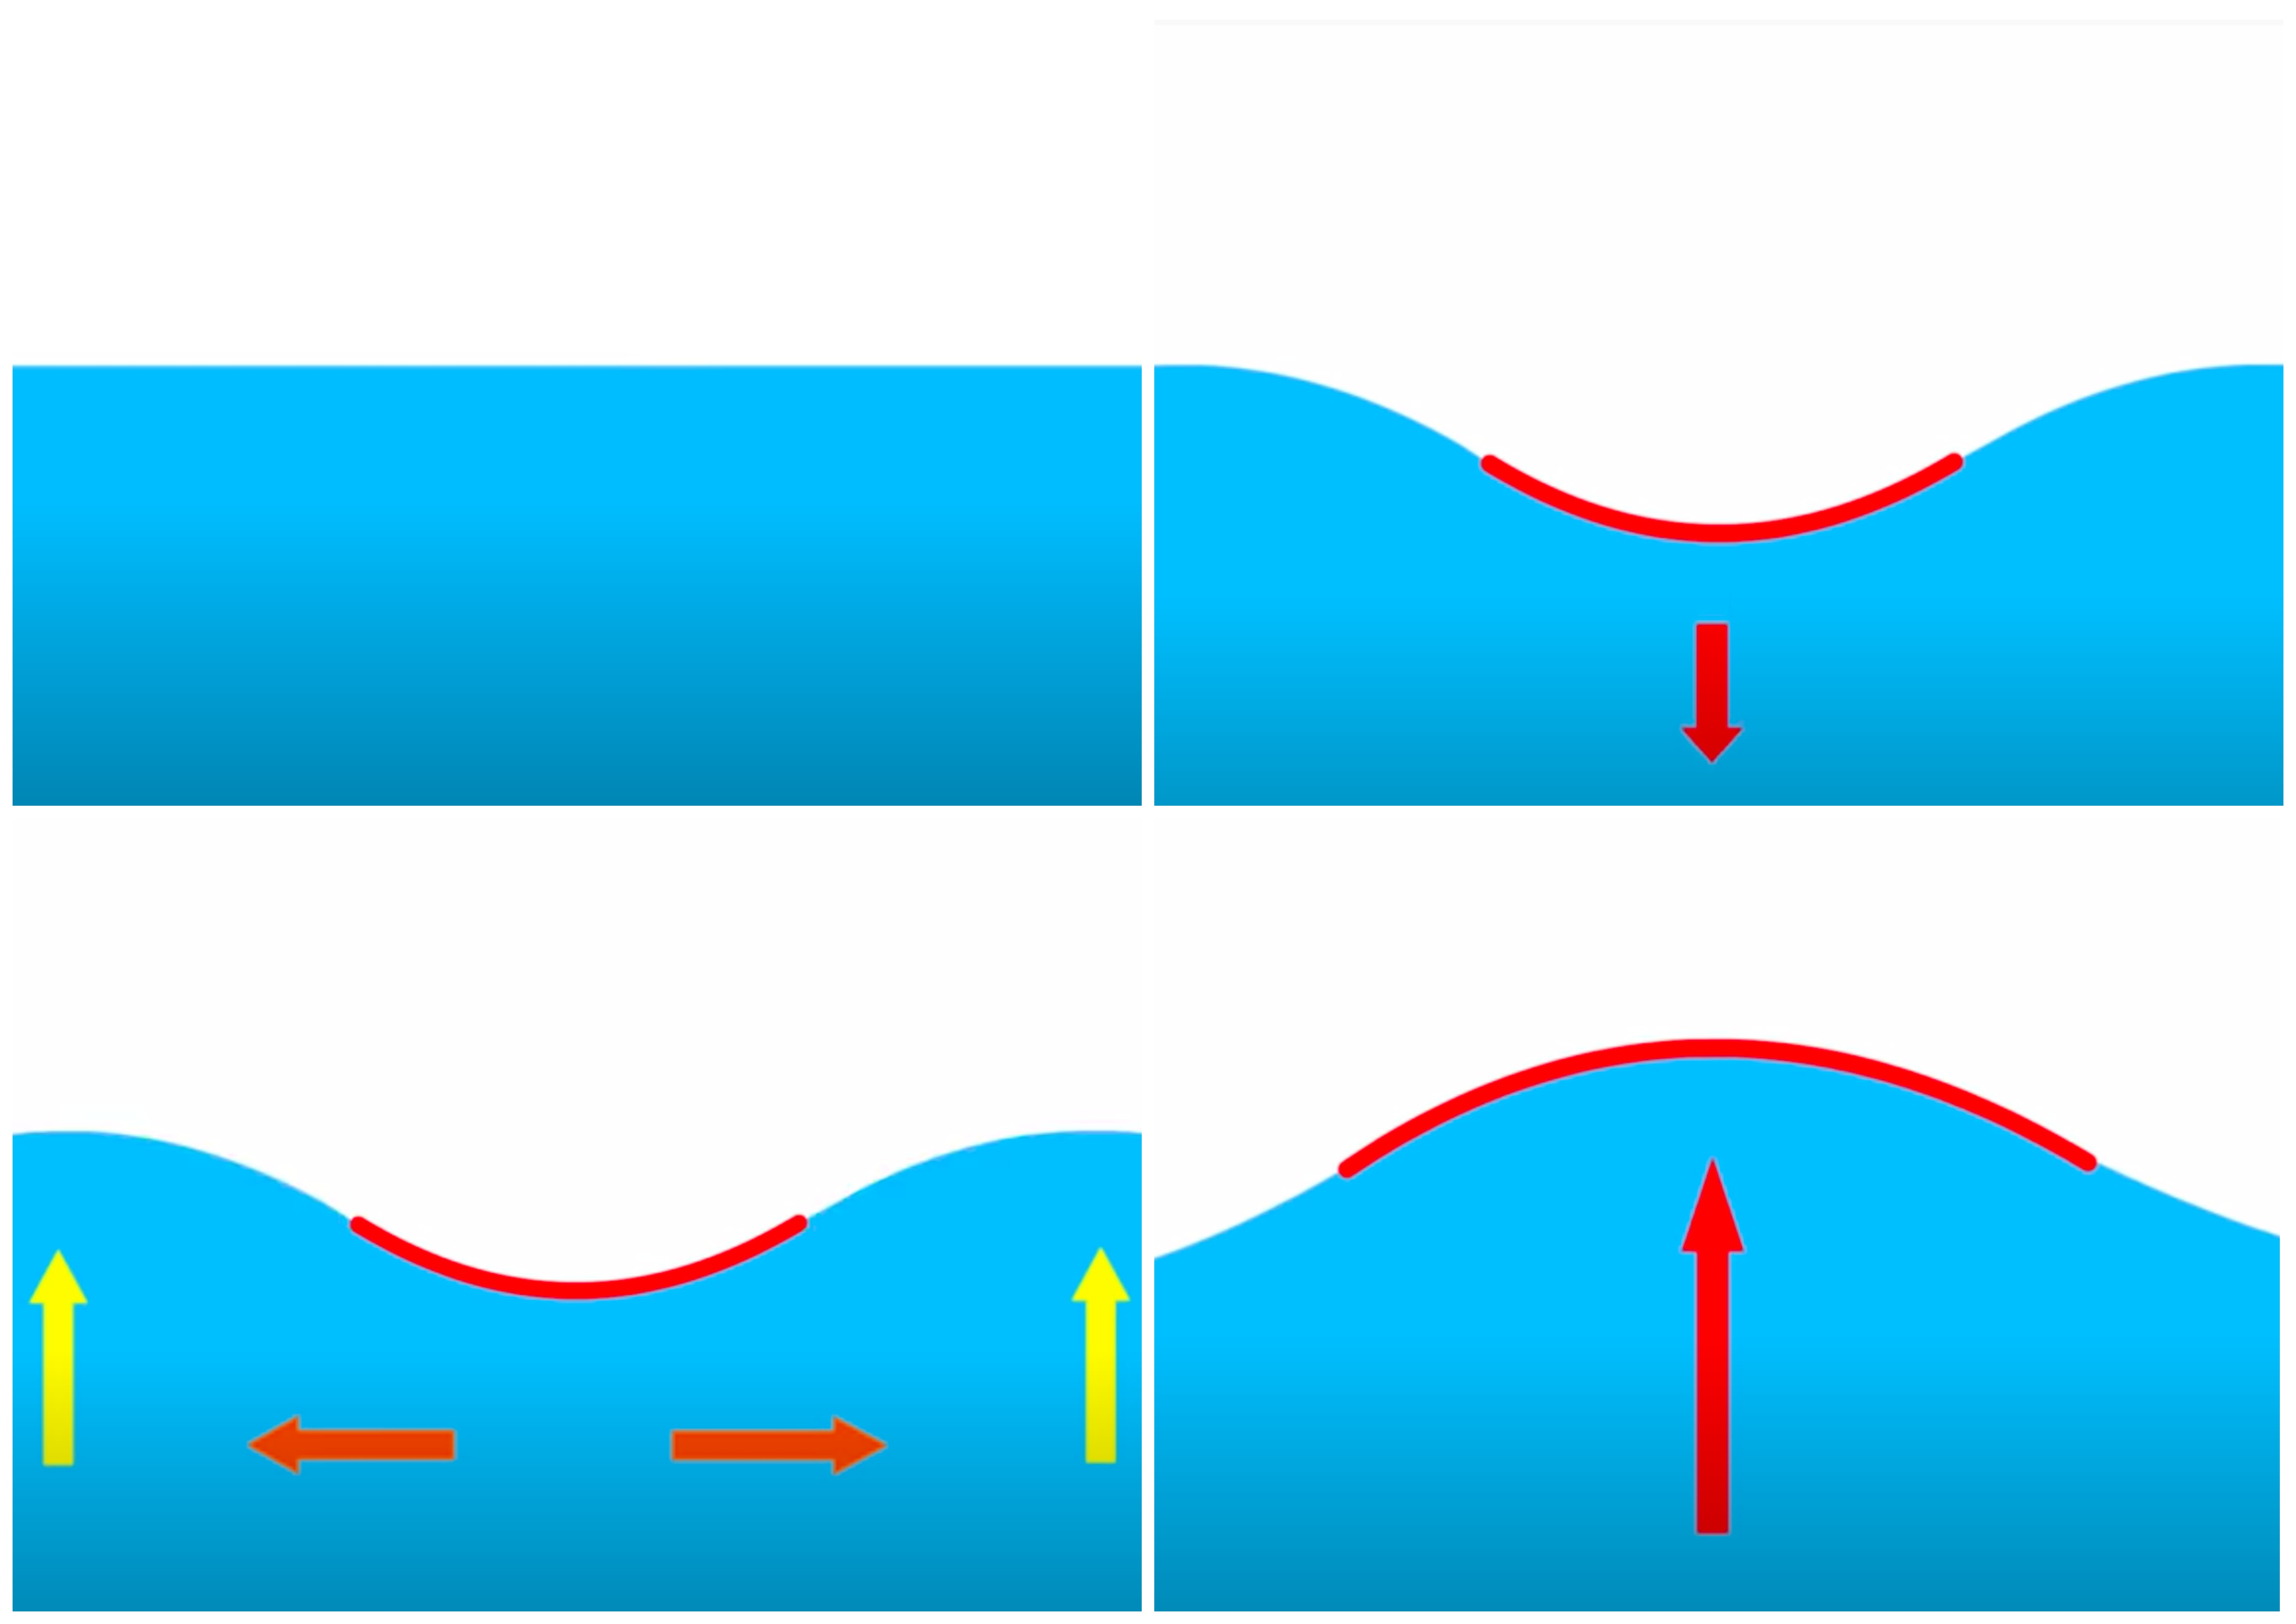
\includegraphics[scale=0.06]{img/wave-process.jpg}
	\end{center}
	\captionsetup{justification=centering}
	\caption{Процесс образования волны.}
	\label{img:wave-process}
\end{figure}

Если восстановить равновесие стремится сила тяжести, то волны называются гравитационными, если сила поверхностного натяжения - капиллярными. Когда силы сопоставимы, волны называют капиллярно-гравитационными. Механизм образования волн подчиняется закону дисперсии. Дисперсия волн - это зависимость скорости распространения волн от их частоты. Именно дисперсия создает сложную картину волн, образованных телом в воде.

В зависимости от требований к результату моделирования выбирается определенный метод визуализации. Так как в центре работы дисперсионные волны, для выполненения поставленных задач необходим такой метод моделирования, при котором выполняется дисперсионное соотношение, т. е. корректно обрабытывается взаимодействие волны и объекта.

\section{Методы визуализации волн}

Существует три группы методов моделирования волн:

\begin{itemize}
    \item процедурные;
    \item методы на основе частиц;
    \item метод поля высот.
\end{itemize}

\subsection{Процедурные методы}

В процедурных методах для представления движения волн используются периодические функции. В ранних работах в качестве такой функции выступала циклоида \cite{orbit-procedure}, далее стали использовать синусоиду \cite{spectrum-darles}. Наложение периодических функций, изменяющихся во времени, создает волновую поверхность. Точка на такой поверхности описывает замкнутую круговую орбиту. Для создания различных волновых эффектов изменяют параметры уравнений орбиты, например, радиус, фазовый угол.

Процедурные методы чаще всего используют при визуализации масштабных волн океана. Преимуществом процедурного моделирования является возможность точно контролировать движение волнового спектра. Недостаток данных методов - сложность получения правильного взаимодействия волн с погруженными телами и границами.  

Выделяют следующие процедурные методы:

\begin{itemize}
    \item метод, основанный на модели Герстнера. Данный метод основан на решении уравнения Эйлера для гравитационных волн. Каждая частица на водной поверхности описывает окружность вокруг положения покоя. Тогда поверхность воды - кривая, которую описывает частица, находящаяся на расстоянии от центра окружности, которая катится по направляющей, как показано на рисунке 1.2. Эту кривую называют трохоидой. Используя лагранжевую систему отсчета находят все необходимые для визуализации параметры волн \cite{orbit-procedure};

\begin{figure}[H]
	\begin{center}
		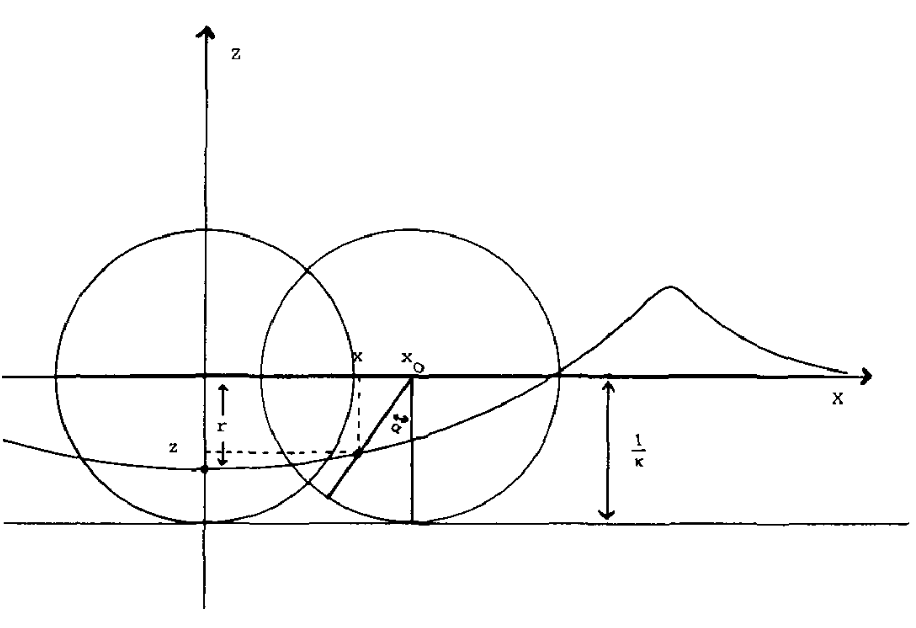
\includegraphics[scale=0.3]{img/trochoid.png}
	\end{center}
	\captionsetup{justification=centering}
	\caption{Поверхность воды представлена трохоидой.}
	\label{img:trochoid}
\end{figure}

    \item спектральные подходы. В данных подходах поверхность океана - поле высот, которое имеет спектр, соответствующий значениям реальной волновой поверхности. Генерируются синусоидальные волны, которые приближенно соответствуют реальным волнам. Если рассматривать функцию представления волны в частотной области, то можно добиться получения трохоид \cite{spectrum-darles}\cite{spectrum-tessendorf}.
\end{itemize}

\subsection{Методы на основе частиц}

В следующих методах моделирования волновой поверхности вода представляется как система частиц. Частицы движутся в соответствии с законами механики и обладают физическими величинами, т. е. задана функция. В определенный момент времени при помощи интерполяции можно получить значение этой функции в произвольной точке.

\begin{figure}[H]
	\begin{center}
		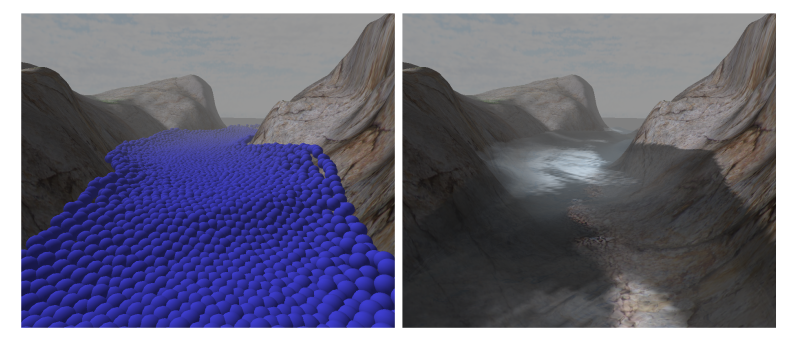
\includegraphics[scale=0.5]{img/particle.png}
	\end{center}
	\captionsetup{justification=centering}
	\caption{Поверхность воды представляется частицами (левый часть рисунка) и отображается в реальном времени (правая часть рисунка). }
	\label{img:particle}
\end{figure}

Для создания реалистичного изображения необходимо большое количество частиц, поэтому даннные методы используются при визуализации небольшого количества воды с неизвестной границей.   

Наиболее распространнёные методы на основе частиц:

\begin{itemize}
    \item гидродинамика сглаженных частиц (SPH). Метод SPH состоит из двух шагов: интерполяции объемов частиц в произвольных положениях и апроксимации пространственных производных. При интерполяции используется сглаживающая функция, называемая ядром, которая является кубическим сплайном. На результат интерполяции оказывают влияние только соседние точки, поэтому необходим поиск только соседних частиц. Так как частицы свободно перемещаются и перемешиваются в пространстве, встает необходимость эффективного решения задачи поиска соседних частиц. Тогда пространство разделяют на ячейки и суммируют по соседним ячейкам. Для большого объема жидкости данный метод создает нереалистичную поверхность \cite{sph};
    \item полунеявный метод движущихся частиц (MPS). Полунеявный метод движущихся частиц основывается на методе расчета движения жидкости Лагранжа. Уравнения движения жидкости дискретизируются с использованием движущихся частиц и их взаимодействий. Далее в методе MPS решается уравнение Навье-Стокса. При использовании данного метода существует возможность добавлять и удалять расчетные точки во время моделирования, поэтому метод является адаптивным. Одной из главных проблем данного метода является создание точных границ при контакте жидкости с твердым предметом или другой жидкостью \cite{mps}.
\end{itemize}

\subsection{Метод поля высот}

В случаях, когда визуализировать необходимо только поверхность воды, а не весь объем водоема, рассматривают волновое уравнение. Волновая поверхность представляется в виде двумерной функции - поля высот \cite{field}. 

Такое упрощение обладает важным преимуществом - снижением вычислительных затрат, что означает повышение скорости моделирования. Кроме того метод поля высот гибко обрабатывает препятствия. Но при такой модели в каждой точке поверхности известно только одно значение высоты, как это показано на рисунке 1.4. Это означает одинаковую скорость распространения всех волн, так, невозможно создать обрушивающиеся волны.

\begin{figure}[H]
	\begin{center}
		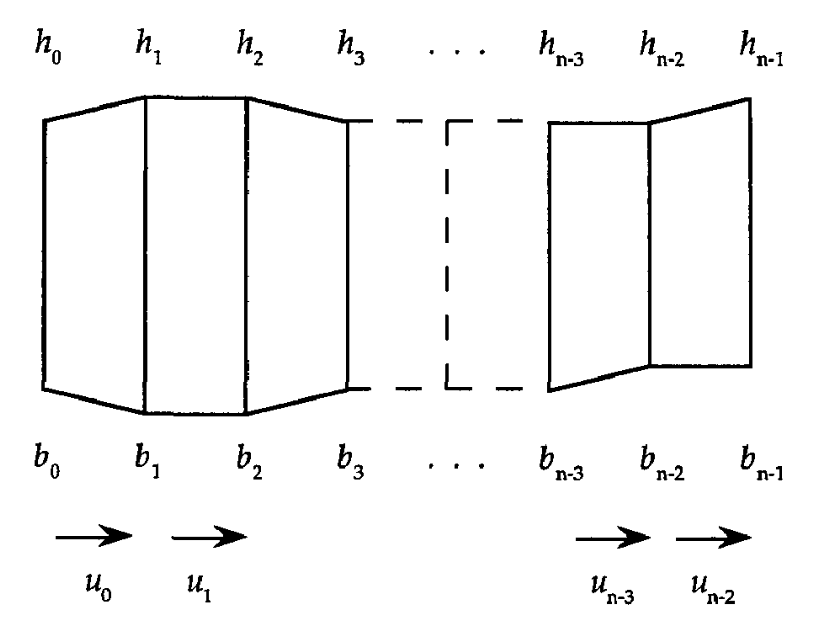
\includegraphics[scale=0.3]{img/height-field.png}
	\end{center}
	\captionsetup{justification=centering}
	\caption{Двумерное представление поверхности воды полями высот h с горизонтальной скоростью u и дна значениями b. }
	\label{img:height-field}
\end{figure}

Комбинация методов поля высот и методов, основанных на частицах, позволяет обходить недостатки отдельных и создавать различные эффекты \cite{shallow}\cite{large-small}.

\section*{Вывод}

Процедурные методы и методы на основе частиц имеют сложности при работе с твердыми телами. Метод поля высот корректно обрабатывает взаимодействие с объектом, причем с более высокой скоростью моделирования. Недостатки метода поля высот не имеют значения при решении выбранной задачи. Моделирование волн будет реализовано при помощи метода поля высот.

\section{Существующие программные обеспечения}

Одним из самых популярных программных обеспечений для работы с трехмерной компьютерной графикой является Blender \cite{blender}. Для моделирования жидкости, в том числе и волн, в Blender существует физическая среда с открытым исходным кодом - Mantaflow \cite{mantaflow}. Данный фреймворк может использоваться с графическим интерфейсом или без него в любой операционной системе. В этом программном продукте реализованы моделирование на основе уравнений Эйлера, гибкие системы частиц, моделирование жидкостей при помощи решателя FLIP, различные эффекты для жидкости, например, поверхностная турбулентность и вейвлет (небольшая рябь). На рисунке 1.5 показано моделирование гибкой системы частиц. 

\begin{figure}[H]
	\begin{center}
		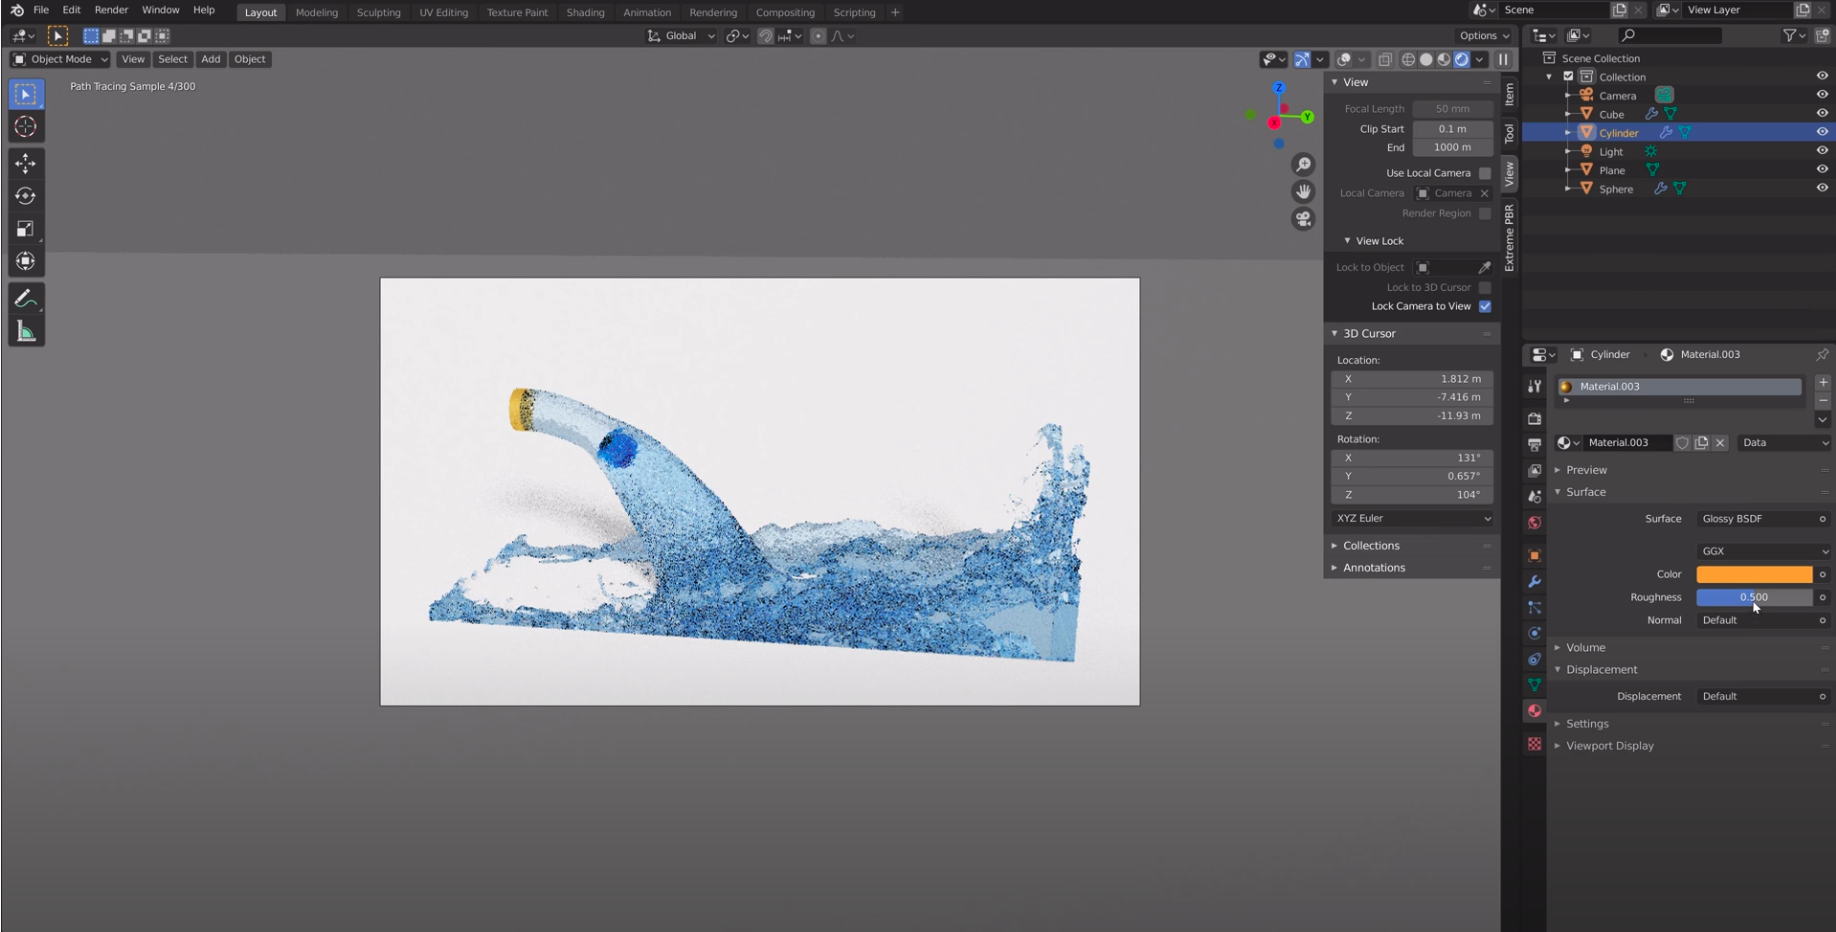
\includegraphics[scale=0.2]{img/mantaflow.png}
	\end{center}
	\captionsetup{justification=centering}
	\caption{Моделирование жидкости в среде Mantaflow в Blender.}
	\label{img:mantaflow}
\end{figure}

В коммерческих и научных проектах используются CFD пакеты. Например, FLOW-3D \cite{flow-3d} представляет набор инструментов для моделирования жидкостей, с целью исследования динамики их движения. Данный пакет позволяет моделировать линейные и нелинейные распространяющиеся поверхностные волны на основе метода конечных объемов. Для визуализации результатов используется программа визуализации FlowSight, как показано на рисунке 1.6.

\begin{figure}[H]
	\begin{center}
		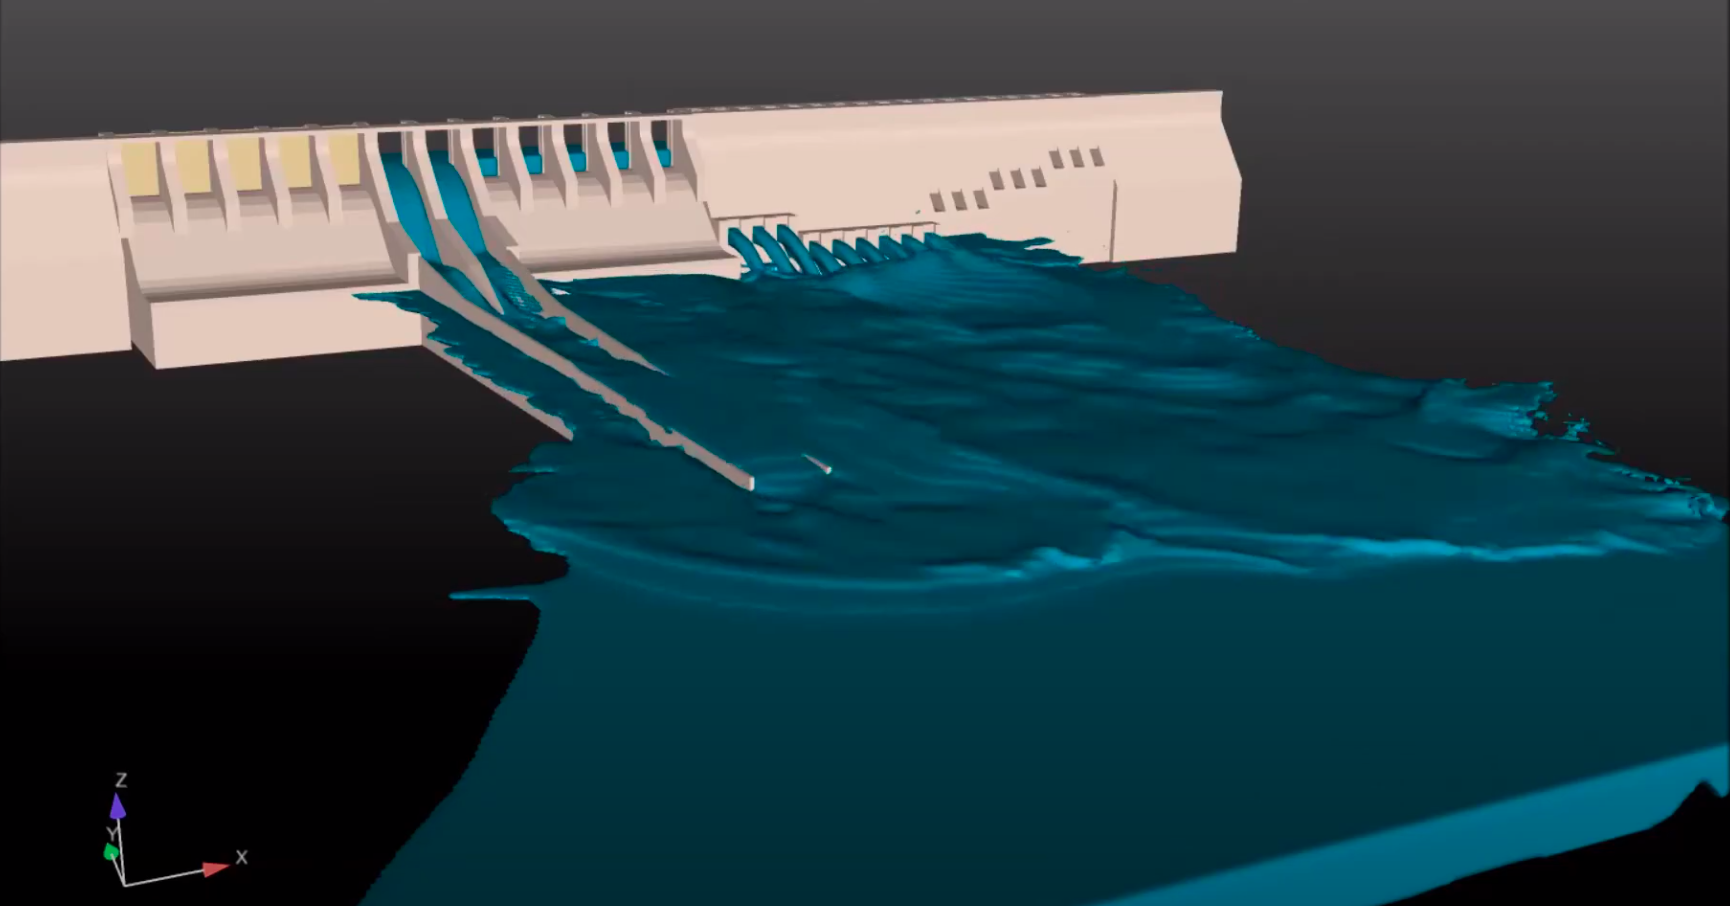
\includegraphics[scale=0.2]{img/flow-3d.png}
	\end{center}
	\captionsetup{justification=centering}
	\caption{Моделирование волн при помощи пакета FLOW-3D.}
	\label{img:flow-3d}
\end{figure}

\section{Модели волны и предмета}

\subsection{Модель волны}

Геометрически волна состоит из следующих элементов, показанных на рисунке 1.7:

\begin{itemize}
	\item гребень - множество точек волны с максимальным положительным отклонением от состояния равновесия;
	\item подошва - множество точек волны с наибольшим отрицательным отклонением от состояния равновесия.
\end{itemize}

\begin{figure}[H]
	\begin{center}
		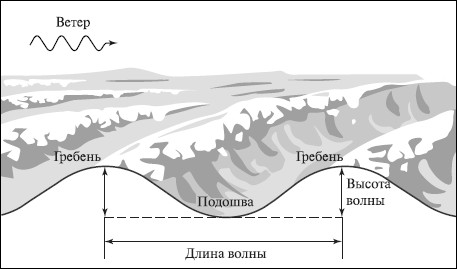
\includegraphics[scale=0.8]{img/wave-elements.jpg}
	\end{center}
	\captionsetup{justification=centering}
	\caption{Геометрическое строение волны.}
	\label{img:wave-elements}
\end{figure}

Кроме того волна обладает следующими параметрами:

\begin{itemize}
	\item высота - вертикальное расстояние от подошвы до гребня;
	\item длина - горизонтальное расстояние от гребня до гребня;
	\item период - временной интервал между прибытием последовательных гребней;
	\item скорость распространения (фазовая скорость).
\end{itemize}

Высота и длина волны указаны на рисунке 1.7.

По математическому описанию волны бывают линейные и нелинейные. Линейные волны обладают небольшой амплитудой, и их свойства описываются волновым уравнением для идеальной субстанции. Нелинейные волны обладают большой амплитудой, что изменяет математическую модель. Так как в центре рассмотрения дисперсионные волны, они обладают линейностью. Модель волны будет основываться на теории волн Эйри (линейной волновой теории) \cite{airy}.

\subsection{Модель предмета}

В центре рассматриваемой системы движения дисперсионных волн, которые образованы в результате контакта поверхности воды с предметом. Для правильной обработки отражения волн от твердых тел важны параметры только той части предмета, которая касается воды.  В связи с этим нет необходимости рассматривать объект детально. Поэтому для его представления требуется такой параметр, как проекция на поверхность воды.

\section{Анализ алгоритмов удаления невидимых линий и поверхностей}

Для выбора подходящего алгоритма удаления невидимых линий и поверхностей необходимо рассмотреть существующие алгоритмы. Главными требованиями при выборе будут скорость работы и отсутствие ограничений к работе с объектами сцены.

\subsection{Алгоритм Робертса}

Алгоритм Робертса работает в объектном пространстве, кроме того работает только с выпуклыми телами. Если тело изначально является не выпуклым, то нужно его разбить на выпуклые составляющие.

Данный алгоритм состоит из следующих основных этапов:

\begin{itemize}
	\item подготовка исходных данных;
	\item удаление линий, экранируемых самим телом;
	\item удаление линий, экранируемых другими телами.
\end{itemize}

Плюсы:

\begin{itemize}
	\item высокая точность вычислений.
\end{itemize}

Минусы:

\begin{itemize}
	\item рост числа трудоемкости алгоритма, как квадрата числа объектов;
	\item работа только с выпуклыми телами.
\end{itemize}

\subsection{Алгоритм, использующий Z-буфер}

Алгоритм Z-буфера решает задачу в пространстве изображений. 

В данном алгоритме рассматривается два буфера. Буфер кадра (регенерации) используется для заполнения атрибутов (интенсивности) каждого пикселя в пространстве изображения. В Z-буфер (буфер глубины) можно помещать информацию о координате z для каждого пикселя.

Для начала необходимо подготовить буферы. Для этого в Z-буфер заносятся максимально возможные значения z, а буфер кадра заполняется значениями пикселя, который описывает фон. Также нужно каждый многоугольник преобразовать в растровую форму и записать в буфер кадра. Сам процесс работы заключается в сравнении глубины каждого нового пикселя, который нужно занести в буфер кадра,
с глубиной того пикселя, который уже занесён в Z-буфер. В зависимости от сравнения принимается решение, нужно ли заносить новый пиксель в буфер кадра и, если нужно, также корректируется Z-буфер (в него нужно занести глубину нового пикселя).

Плюсы:

\begin{itemize}
	\item произвольная сложность сцены;
	\item поскольку размеры изображения ограничены размером экрана дисплея, трудоемкость алгоритма зависит линейно от числа рассматриваемых поверхностей;
	\item элементы сцены заносятся в буфер кадра в произвольном порядке, поэтому в данном алгоритме не тратится время на выполнение сортировок.
\end{itemize}

Минусы:

\begin{itemize}
	\item большой объем требуемой памяти;
	\item трудоемкость устранения лестничного эффекта;
	\item трудности реализации эффектов прозрачности.
\end{itemize}

\subsection{Алгоритм обратной трассировки}

Алгоритм обратной трассировки лучей отслеживает лучи в обратном направлении (от наблюдателя к объекту). Считается, что наблюдатель расположен на положительной полуоси z в бесконечности, поэтому все световые лучи параллельны оси z. В ходе работы испускаются лучи от наблюдателя и ищутся пересечения луча и всех объектов сцены.
В результате, пересечение с максимальным значением z является видимой частью поверхности, и атрибуты данного объекта используются для определения характеристик пикселя, через центр которого проходит данный световой луч. 

Эффективность процедуры определения пересечений луча с поверхностью объекта оказывает самое большое влияние на эффективность всего алгоритма. Чтобы избавиться от ненужного поиска пересечений было придумано искать пересечение луча с объемной оболочкой рассматриваемого объекта. Под оболочкой понимается некоторый простой объект, внутрь которого можно поместить рассматриваемый объект, к примеру параллелепипед или сферу. 

В дальнейшем при рассмотрении пересечения луча и объемной оболочкой рассматриваемого объекта, если такого пересечения нет, то и соответственно пересечения луча и самого рассматриваемого объекта нет, и наоборот, пересечение найдено, то возможно, есть пересечение луча и рассматриваемого объекта. 

Для расчета эффектов освещения сцены проводятся вторичные лучи от точек пересечения ко всем источникам света. Если на пути этих лучей встречается непрозрачное тело, значит данная точка находится в тени, иначе он влияет на освещение данной точки. Также для получения более реалистичного изображения сцены, нужно учитывать вклады отраженных и преломленных лучей.

Плюсы:

\begin{itemize}
	\item возможность использования алгоритма в параллельных вычислительных системах.
\end{itemize}

Минусы:

\begin{itemize}
	\item производительность алгоритма.
\end{itemize}

\subsection*{Вывод}

Для удаления невидимых линий и поверхностей выбран алгоритм Z-буфера, так как обладает важными преимуществами - высокой скоростью работы и произвольной сложностью сцены.

\section{Анализ методов закрашивания}

Методы закрашивания используются для затенения полигонов (или по-
верхностей, аппроксимированных полигонами) в условиях некоторой сцены, имеющей источники освещения.

\subsection{Простая закраска}

Одной из самых простых моделей освещения является модель Ламберта. Она учитывает только идеальное диффузное отражение света от тела. Считается, что свет падающий в точку, одинаково рассеивается по всем направлениям полупространства. Таким образом, освещенность в точке определяется только плотностью света в точке поверхности, а она линейно зависит от косинуса угла падения. При этом положение наблюдателя не имеет значение, т.к. диффузно отраженный свет рассеивается равномерно по всем направлениям.

Большим недостатком данной модели является то, что согласно приведённой выше формуле, все точки грани будут иметь одинаковую интенсивность.

\subsection{Закраска по Гуро}

Данный алгоритм предполагает следующие шаги:

\begin{itemize}
	\item вычисление векторов нормалей к каждой грани;
    \item вычисление векторов нормали к каждой вершине грани путем усреднения нормалей к граням;
    \item вычисление интенсивности в вершинах грани;
    \item интерполяция интенсивности вдоль ребер грани;
    \item линейная интерполяция интенсивности вдоль сканирующей строки.
\end{itemize}

Плюсы:

\begin{itemize}
	\item хорошо сочетается с диффузным отражением;
	\item изображение получается более реалистичным.
\end{itemize}

Минусы:

\begin{itemize}
	\item данный метод интерполяции обеспечивает лишь непрерывность значений интенсивности вдоль границ многоугольников, но не обеспечивает непрерывность изменения интенсивности.
\end{itemize}


\subsection{Закраска по Фонгу}

При такой закраске, в отличие от метода Гуро, вдоль сканирующей строки интерполируется значение вектора нормали, а не интенсивности. 

Шаги алгоритма:

\begin{itemize}
    \item вычисление векторов нормалей в каждой грани.
    \item вычисление векторов нормали к каждой вершине грани.
    \item интерполяция векторов нормалей вдоль ребер грани.
    \item линейная интерполяция векторов нормалей вдоль сканирующей строки.
    \item вычисление интенсивности в очередной точке сканирующей строки.
\end{itemize}

Плюсы:

\begin{itemize}
	\item можно достичь лучшей локальной аппроксимации кривизны поверхности.
\end{itemize}

Минусы:

\begin{itemize}
	\item ресурсоемкость;
	\item вычислительная сложность.
\end{itemize}

\subsection*{Вывод}

Для закрашивания выбран алгоритм Гуро, так как данный алгоритм обладает важным преимуществом - высокой реалистичностью изображения.

\section*{Вывод}

В данном разделе были формально описаны модели волны и
предметы, были рассмотрены алгоритмы удаления невидимых линий и поверхностей, методы закрашивания поверхностей. В качестве алгоритма моделирования дисперсионных волн был выбран метод поля высот, в качестве алгоритма удаления невидимых линий и поверхностей был выбран алгоритм z-буфера, в качестве метода закрашивания был выбран алгоритм закраски Гуро.